\chapter{树}

\section{二叉树的遍历} %%%%%%%%%%%%%%%%%%%%%%%%%%%%%%
\label{sec:binaryTreeTraversal}

在中序遍历中,一个节点的前驱,是其左子树的最右下角结点,后继,是其右子树的最左下角结点。

在后序遍历中,
\begindot
\item 若结点是根结点,则其后继为空;
\item 若结点是双亲的右子树,或是左子树但双亲无右子树,则其后继为双亲结点;
\item 若结点是双亲的左子树且双亲有右子树,则其后继为右子树按后序遍历的第一个结点
\myenddot


\begin{Codex}[label=binary_tree.cpp]
#include <stack>
#include <queue>

 /*
  *@struct
  *@brief 二叉树结点
  */
typedef struct binary_tree_node_t {
    binary_tree_node_t *lchild;   /* 左孩子*/
    binary_tree_node_t *rchild;   /* 右孩子*/
    void* data; /* 结点的数据*/
}binary_tree_node_t;

/** 
  * @brief 先序遍历,递归.
  * @param[in] root 根结点
  * @param[in] visit 访问数据元素的函数指针
  * @return 无
  */
void pre_order_r(const binary_tree_node_t *root, 
                 int (*visit)(void*)) {
    if(root != NULL) {
        (void)visit(root->data);
        pre_order_r(root->lchild, visit);
        pre_order_r(root->rchild, visit);
    }
}

/** 
  * @brief 中序遍历,递归.
  */
void in_order_r(const binary_tree_node_t *root, 
                int (*visit)(void*)) {
    if(root != NULL) {
        in_order_r(root->lchild, visit);
        (void)visit(root->data);
        in_order_r(root->rchild, visit);
    }
}

/** 
  * @brief 后序遍历,递归.
  */
void post_order_r(const binary_tree_node_t *root, 
                  int (*visit)(void*)) {
    if(root != NULL) {
        post_order_r(root->lchild, visit);
        post_order_r(root->rchild, visit);
        (void)visit(root->data);
    }
}

/** 
 * @brief 先序遍历,非递归.
 */
void pre_order(const binary_tree_node_t *root, 
               int (*visit)(void*)) {
    const binary_tree_node_t *p;
    std::stack<const binary_tree_node_t *> s;

    p = root;

    if(p != NULL) {
        s.push(p);
    }

    while(!s.empty()) {
        p = s.top();
        s.pop();
        visit(p->data);
        if(p->rchild != NULL) {
            s.push(p->rchild);
        }
        if(p->lchild != NULL) {
            s.push(p->lchild);
        }
    }
}

/** 
 * @brief 中序遍历,非递归.
 */
void in_order(const binary_tree_node_t *root, 
              int (*visit)(void*)) {
    const binary_tree_node_t *p;
    std::stack<const binary_tree_node_t *> s;

    p = root;

    while(!s.empty() || p!=NULL) {
        if(p != NULL) {
            s.push(p);
            p = p->lchild;
        } else {
            p = s.top();
            s.pop();
            visit(p->data);
            p = p->rchild;
        }
    }
}

/** 
 * @brief 后序遍历,非递归.
 */
void post_order(const binary_tree_node_t *root, 
                int (*visit)(void*)) {
    /* p,正在访问的结点,q,刚刚访问过的结点*/
    const binary_tree_node_t *p, *q;
    std::stack<const binary_tree_node_t *> s;

    p = root;

    do {
        while(p != NULL) { /* 往左下走*/
            s.push(p);
            p = p->lchild;
        }
        q = NULL;
        while(!s.empty()) {
            p = s.top();
            s.pop();
            /* 右孩子不存在或已被访问,访问之*/
            if(p->rchild == q) {
                visit(p->data);
                q = p; /* 保存刚访问过的结点*/
            } else {
                /* 当前结点不能访问,需第二次进栈*/
                s.push(p);
                /* 先处理右子树*/
                p = p->rchild;
                break;
            }
        }
    }while(!s.empty());
}

/** 
 * @brief 层次遍历,也即BFS.
 *
 * 跟先序遍历一模一样,唯一的不同是栈换成了队列
 */
void level_order(const binary_tree_node_t *root, 
                 int (*visit)(void*)) {
    const binary_tree_node_t *p;
    std::queue<const binary_tree_node_t *> q;

    p = root;

    if(p != NULL) {
        q.push(p);
    }

    while(!q.empty()) {
        p = q.front();
        q.pop();
        visit(p->data);
        if(p->lchild != NULL) { /*先左后右或先右后左无所谓*/
            q.push(p->lchild);
        }
        if(p->rchild != NULL) {
            q.push(p->rchild);
        }
    }
}
\end{Codex}

\section{线索二叉树} %%%%%%%%%%%%%%%%%%%%%%%%%%%%%%
二叉树中存在很多空指针,可以利用这些空指针,指向其前驱或者后继。这种利用起来的空指针称为线索,这种改进后的二叉树称为线索二叉树(threaded binary tree)。

一棵n个结点的二叉树含有n+1个空指针。这是因为,假设叶子节点数为$n_0$,度为1的节点数为$n_1$,度为2的节点数为$n_2$,每个叶子节点有2个空指针,每个度为1的节点有1个空指针,则空指针的总数为$2n_0+n_1$,又有$n_0=n_2+1$(留给读者证明),因此空指针总数为$2n_0+n_1=n_0+n_2+1+n_1=n_0+n_1+n_2+1=n+1$。

在二叉树线索化过程中,通常规定,若无左子树,令lchild指向前驱,若无右子树,令rchild指向后继。还需要增加两个标志域表示当前指针是不是线索,例如ltag=1,表示lchild指向的是前驱,ltag=0,表示lchild指向的是左孩子,rtag类似。

二叉树的线索化,实质上就是遍历一棵树,只是在遍历的过程中,检查当前节点的左右指针是否为空,若为空,将它们改为指向前驱或后继的线索。

以中序线索二叉树为例,指针pre表示前驱,succ表示后继,如图~\ref{fig:threadedBinaryTree}所示。

\begin{center}
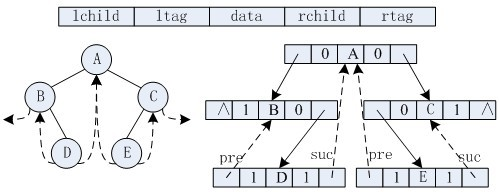
\includegraphics[width=300pt]{threaded-binary-tree.png} \\
\figcaption{中序线索二叉树}\label{fig:threadedBinaryTree}
\end{center}

在中序线索二叉树中,一个节点的前驱,是其左子树的最右下角结点,后继,是其右子树的最左下角结点。

中序线索二叉树的C语言实现如下。
\begin{Codex}[label=theaded_binary_tree.c]
/** @file threaded_binary_tree.c
  * @brief 线索二叉树.
  * @author soulmachine@gmail.com
  * @date 2013-06-16
  */
#include <stddef.h>    /* for NULL */
#include <stdio.h>

/* 结点数据的类型. */
typedef int elem_t;

 /**
  *@struct
  *@brief 线索二叉树结点.
  */
typedef struct tbt_node_t {
    int ltag; /** 1表示是线索,0表示是孩子 */
    int rtag; /** 1表示是线索,0表示是孩子 */
    struct tbt_node_t *lchild; /** 左孩子*/
    struct tbt_node_t *rchild; /** 右孩子*/
    elem_t data; /** 结点所存放的数据*/
}tbt_node_t;

/* 内部函数 */
static void in_thread(tbt_node_t *p, tbt_node_t **pre);
static tbt_node_t *first(tbt_node_t *p);
static tbt_node_t *next(const tbt_node_t *p);

 /**
  * @brief 建立中序线索二叉树.
  * @param[in] root 树根
  * @return 无
  */
void create_in_thread(tbt_node_t *root) {
    /* 前驱结点指针*/
    tbt_node_t *pre=NULL;
    if(root != NULL) { /* 非空二叉树,线索化*/
        /* 中序遍历线索化二叉树*/
        in_thread(root, &pre);
        /* 处理中序最后一个结点*/
        pre->rchild = NULL;
        pre->rtag = 1;
    }
}


/**
  * @brief 在中序线索二叉树上执行中序遍历.
  * @param[in] root 树根
  * @param[in] visit 访问结点的数据的函数
  * @return 无
  */
void in_order(tbt_node_t *root, int(*visit)(elem_t*)) {
    tbt_node_t *p;
    for(p = first(root); p != NULL; p = next(p)) {
        (void)visit(&(p->data));
    }
}


 /*
  * @brief 中序线索化二叉树的主过程.
  * @param[in] p 当前要处理的结点
  * @param[inout] pre 当前结点的前驱结点
  * @return 无
  */
static void in_thread(tbt_node_t *p, tbt_node_t **pre) {
    if(p != NULL) {
        in_thread(p->lchild, pre); /* 线索化左子树 */
        if(p->lchild == NULL) {  /* 左子树为空,建立前驱 */
            p->lchild = *pre;
            p->ltag = 1;
        }
        /* 建立前驱结点的后继线索 */
        if((*pre) != NULL &&
            (*pre)->rchild == NULL) {
            (*pre)->rchild = p;
            (*pre)->rtag = 1;
        }
        *pre = p; /* 更新前驱 */
        in_thread(p->rchild, pre); /* 线索化右子树 */
    }
}

 /*
  * @brief 寻找线索二叉树的中序下的第一个结点.
  * @param[in] p 线索二叉树中的任意一个结点
  * @return 此线索二叉树的第一个结点
  */
static tbt_node_t *first(tbt_node_t *p) {
    if(p == NULL)  return NULL;

    while(p->ltag == 0) {
        p = p->lchild;  /* 最左下结点,不一定是叶结点*/
    }
    return p;
}

 /*
  * @brief 求中序线索二叉树中某结点的后继.
  * @param[in] p 某结点
  * @return p的后继
  */
static tbt_node_t *next(const tbt_node_t *p) {
    if(p->rtag == 0) {
        return first(p->rchild);
    } else {
        return p->rchild;
    }
}
\end{Codex}

中序线索二叉树最简单,在中序线索的基础上稍加修改就可以实现先序,后续就要再费点心思了。


\section{Morris Traversal} %%%%%%%%%%%%%%%%%%%%%%%%%%%%%%
通过前面第\S \ref{sec:binaryTreeTraversal}节,我们知道,实现二叉树的前序(preorder)、中序(inorder)、后序(postorder)遍历有两个常用的方法,一是递归(recursive),二是栈(stack+iterative)。这两种方法都是O(n)的空间复杂度。

而Morris Traversal只需要O(1)的空间复杂度。这种算法跟线索二叉树很像,不过Morris Traversal一边建线索,一边访问数据,访问完后销毁线索,保持二叉树不变。

\subsection{Morris中序遍历}
Morris中序遍历的步骤如下:
\begin{enumerate}
\item 初始化当前节点cur为root节点
\item 如果cur没有左孩子,则输出当前节点并将其右孩子作为当前节点,即cur = cur->rchild。
\item 如果cur有左孩子,则寻找cur的前驱,即cur的左子树的最右下角结点。\\
   a) 如果前驱节点的右孩子为空,将它的右孩子指向当前节点,当前节点更新为当前节点的左孩子。\\
   b) 如果前驱节点的右孩子为当前节点,将它的右孩子重新设为空(恢复树的形状),输出当前节点,当前节点更新为当前节点的右孩子。
\item 重复2、3步骤,直到cur为空。
\end{enumerate}
如图~\ref{fig:inorderMorris}所示,cur表示当前节点,深色节点表示该节点已输出。

\begin{center}
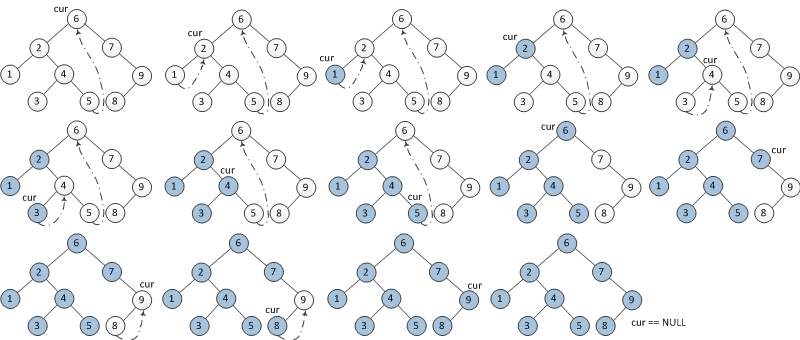
\includegraphics[width=360pt]{inorder-morris-traversal.png} \\
\figcaption{Morris中序遍历}\label{fig:inorderMorris}
\end{center}

C语言实现见第\S\ref{sec:morrisTraversalImpl}节。

\subsubsection{相关的题目}
\begindot
\item Leet Code - Binary Tree Inorder Traversal, \myurl{http://leetcode.com/onlinejudge\#question_94}
\myenddot


\subsection{Morris先序遍历}
Morris先序遍历的步骤如下:
\begin{enumerate}
\item 初始化当前节点cur为root节点
\item 如果cur没有左孩子,则输出当前节点并将其右孩子作为当前节点,即cur = cur->rchild。
\item 如果cur有左孩子,则寻找cur的前驱,即cur的左子树的最右下角结点。\\
   a) 如果前驱节点的右孩子为空,将它的右孩子指向当前节点,\textbf{输出当前节点(在这里输出,这是与中序遍历唯一的不同点)}当前节点更新为当前节点的左孩子。\\
   b) 如果前驱节点的右孩子为当前节点,将它的右孩子重新设为空(恢复树的形状),\sout{输出当前节点,}当前节点更新为当前节点的右孩子。
\item 重复2、3步骤,直到cur为空。
\end{enumerate}
如图~\ref{fig:preorderMorris}所示。

\begin{center}
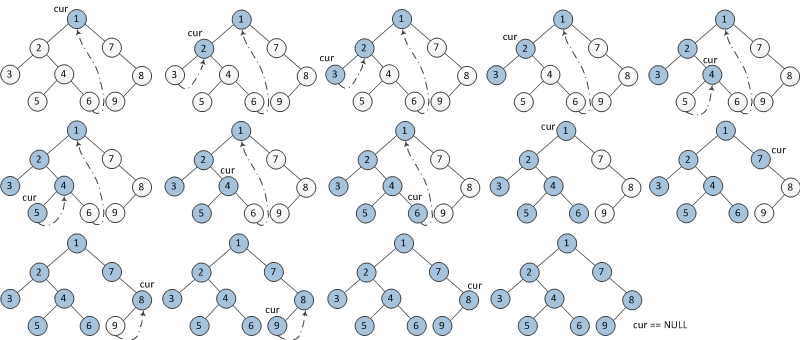
\includegraphics[width=360pt]{preorder-morris-traversal.png} \\
\figcaption{Morris先序遍历}\label{fig:preorderMorris}
\end{center}

C语言实现见第\S\ref{sec:morrisTraversalImpl}节。


\subsection{Morris后序遍历}
Morris后续遍历稍微复杂,需要建立一个临时节点dump,令其左孩子是root,并且还需要一个子过程,就是倒序输出某两个节点之间路径上的所有节点。

Morris后序遍历的步骤如下:
\begin{enumerate}
\item 初始化当前节点cur为root节点
\item 如果cur没有左孩子,则\sout{输出当前节点并}将其右孩子作为当前节点,即cur = cur->rchild。
\item 如果cur有左孩子,则寻找cur的前驱,即cur的左子树的最右下角结点。\\
   a) 如果前驱节点的右孩子为空,将它的右孩子指向当前节点,当前节点更新为当前节点的左孩子。\\
   b) 如果前驱节点的右孩子为当前节点,将它的右孩子重新设为空(恢复树的形状),\sout{输出当前节点,}\textbf{倒序输出从当前节点的左孩子到该前驱节点这条路径上的所有节点。}当前节点更新为当前节点的右孩子。
\item 重复2、3步骤,直到cur为空。
\end{enumerate}
如图~\ref{fig:postorderMorris}所示。

\begin{center}
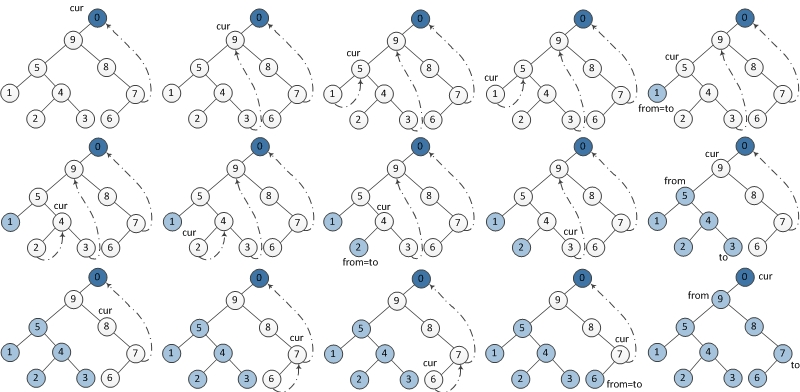
\includegraphics[width=360pt]{postorder-morris-traversal.png} \\
\figcaption{Morris后序遍历}\label{fig:postorderMorris}
\end{center}

C语言实现见第\S\ref{sec:morrisTraversalImpl}节。


\subsection{C语言实现}
\label{sec:morrisTraversalImpl}
\begin{Codex}[label=morris_traversal.cpp]
/** @file morris_traversal.c
 * @brief Morris遍历算法.
 * @author soulmachine@gmail.com
 * @date 2013-06-16
 */
#include<stdio.h>
#include<stdlib.h>

/* 结点数据的类型. */
typedef int elem_t;

/**
 *@struct
 *@brief 二叉树结点.
 */
typedef struct bt_node_t {
    elem_t data; /* 节点的数据 */
    struct bt_node_t *lchild; /* 左孩子 */
    struct bt_node_t *rchild; /* 右孩子 */
} bt_node_t;

/**
 * @brief 中序遍历,Morris算法.
 * @param[in] root 根节点
 * @param[in] visit 访问函数
 * @return 无
 */
void in_order_morris(bt_node_t *root, int(*visit)(elem_t*)) {
    bt_node_t *cur, *pre;

    cur = root;
    while (cur != NULL ) {
        if (cur->lchild == NULL ) {
            visit(cur->data);
            cur = cur->rchild;
        } else {
            /* 查找前驱 */
            pre = cur->lchild;
            while (pre->rchild != NULL && pre->rchild != cur)
                pre = pre->rchild;

            if (pre->rchild == NULL ) {    /* 还没线索化,则建立线索 */
                pre->rchild = cur;
                cur = cur->lchild;
            } else {    /* 已经线索化,则访问节点,并删除线索  */
                visit(cur->data);
                pre->rchild = NULL;
                cur = cur->rchild;
            }
        }
    }
}

/**
 * @brief 先序遍历,Morris算法.
 * @param[in] root 根节点
 * @param[in] visit 访问函数
 * @return 无
 */
void pre_order_morris(bt_node_t *root, int (*visit)(elem_t*)) {
    bt_node_t *cur = root, *pre = NULL;
    while (cur != NULL ) {
        if (cur->lchild == NULL ) {
            visit(cur->data);
            cur = cur->rchild;
        } else {
            pre = cur->lchild;
            while (pre->rchild != NULL && pre->rchild != cur)
                pre = pre->rchild;

            if (pre->rchild == NULL ) {
                visit(cur->data);  // 仅这一行与中序不同
                pre->rchild = cur;
                cur = cur->lchild;
            } else {
                pre->rchild = NULL;
                cur = cur->rchild;
            }
        }
    }
}

static void reverse(bt_node_t *from, bt_node_t *to);
static void visit_reverse(bt_node_t* from, bt_node_t *to, int (*visit)(elem_t*));
/**
 * @brief 后序遍历,Morris算法.
 * @param[in] root 根节点
 * @param[in] visit 访问函数
 * @return 无
 */
void post_order_morris(bt_node_t *root, int (*visit)(elem_t*)) {
    bt_node_t dump = { 0, NULL, NULL };
    dump.lchild = root;
    bt_node_t *cur = &dump, *pre = NULL;
    while (cur != NULL ) {
        if (cur->lchild == NULL ) {
            cur = cur->rchild;
        } else {
            pre = cur->lchild;
            while (pre->rchild != NULL && pre->rchild != cur)
                pre = pre->rchild;

            if (pre->rchild == NULL ) {
                pre->rchild = cur;
                cur = cur->lchild;
            } else {
                visit_reverse(cur->lchild, pre, visit);  // call print
                pre->rchild = NULL;
                cur = cur->rchild;
            }
        }
    }
}

/*
 * @brief 逆转路径.
 * @param[in] from from
 * @param[to] to to
 * @return 无
 */
static void reverse(bt_node_t *from, bt_node_t *to) {
    if (from == to) return;
    bt_node_t *x = from, *y = from->rchild, *z;
    while (x != to) {
        z = y->rchild;
        y->rchild = x;
        x = y;
        y = z;
    }
}

/*
 * @brief  访问逆转后的路径上的所有结点.
 * @param[in] from from
 * @param[to] to to
 * @return 无
 */
static void visit_reverse(bt_node_t* from, bt_node_t *to, int (*visit)(elem_t*)) {
    reverse(from, to);

    bt_node_t *p = to;
    while (1) {
        visit(p->data);
        if (p == from)
            break;
        p = p->rchild;
    }

    reverse(to, from);
}

/*
 * @brief 分配一个新节点.
 * @param[in] data 新节点的数据
 * @return 新节点
 */
bt_node_t* new_node(int data) {
    bt_node_t* node = (bt_node_t*) malloc(sizeof(bt_node_t));
    node->data = data;
    node->lchild = NULL;
    node->rchild = NULL;

    return (node);
}

static int print(const elem_t *data) {
    printf(" %d ", data);
    return 0;
}

/* test */
int main() {
    /* 构造的二叉树如下
       1
     /   \
    2      3
  /  \
4     5
     */
    bt_node_t *root = new_node(1);
    root->lchild = new_node(2);
    root->rchild = new_node(3);
    root->lchild->lchild = new_node(4);
    root->lchild->rchild = new_node(5);

    in_order_morris(root, print);
    printf("\n");
    pre_order_morris(root, print);
    printf("\n");
    post_order_morris(root, print);

    return 0;
}
\end{Codex}


\section{重建二叉树} %%%%%%%%%%%%%%%%%%%%%%%%%%%%%%
\begin{Codex}[label=binary_tree_rebuild.c]
#include <stdio.h>
#include <stdlib.h>
#include <string.h>
#include <stddef.h>
/**
 * @brief 给定前序遍历和中序遍历,输出后序遍历.
 *
 * @param[in] pre 前序遍历的序列
 * @param[in] in 中序遍历的序列
 * @param[in] n 序列的长度
 * @param[out] post 后续遍历的序列
 * @return 无
 */
void build_post(const char * pre, const char *in, const int n, char *post) {
    if(n <= 0) return;
    int left_len = strchr(in, pre[0]) - in;
    build_post(pre + 1, in, left_len, post);
    build_post(pre + left_len + 1, in + left_len + 1,
            n - left_len - 1, post + left_len);
    post[n - 1] = pre[0];
}

#define MAX  64
// 测试
// BCAD CBAD,输出 CDAB
// DBACEGF ABCDEFG,输出 ACBFGED
void build_post_test() {
    char pre[MAX] = {0};
    char in[MAX] = {0};
    char post[MAX] = {0};
    scanf("%s%s", pre, in);

    const int n = strlen(pre);
    build_post(pre, in, n, post);
    printf("%s\n", post);
}

/* 结点数据的类型. */
typedef char elem_t;

/**
 *@struct
 *@brief 二叉树结点.
 */
typedef struct bt_node_t {
    elem_t data; /* 节点的数据 */
    struct bt_node_t *lchild; /* 左孩子 */
    struct bt_node_t *rchild; /* 右孩子 */
} bt_node_t;

/**
 * @brief 给定前序遍历和中序遍历,重建二叉树.
 *
 * @param[in] pre 前序遍历的序列
 * @param[in] in 中序遍历的序列
 * @param[in] n 序列的长度
 * @param[out] root 根节点
 * @return 无
 */
void rebuild(const char *pre, const char *in, int n, bt_node_t **root) {
    // 检查终止条件
    if (n <= 0 || pre == NULL || in == NULL)
        return;
    //获得前序遍历的第一个结点
    *root = (bt_node_t*) malloc(sizeof(bt_node_t));
    (*root)->data = *pre;
    (*root)->lchild = NULL;
    (*root)->rchild = NULL;

    int left_len = strchr(in, pre[0]) - in;
    //重建左子树
    rebuild(pre + 1, in, left_len, &((*root)->lchild));
    //重建右子树
    rebuild(pre + left_len + 1, in + left_len + 1, n - left_len - 1,
            &((*root)->rchild));
}

void print_post_order(const bt_node_t *root) {
    if(root != NULL) {
        print_post_order(root->lchild);
        print_post_order(root->rchild);
        printf("%c", root->data);
    }
}

void rebuild_test() {
    char pre[MAX] = { 0 };
    char in[MAX] = { 0 };
    scanf("%s%s", pre, in);
    const int n = strlen(pre);

    bt_node_t *root;
    rebuild(pre, in, n, &root);
    print_post_order(root);
}

int main() {
    build_post_test();
    rebuild_test();
    return 0;
}
\end{Codex}


\section{堆} %%%%%%%%%%%%%%%%%%%%%%%%%%%%%%

\subsection{原理和实现}
C++可以直接使用\fn{std::priority_queue}。

\begin{Codex}[label=heap.c]
/** @file heap.c
 * @brief 堆,默认为小根堆,即堆顶为最小.
 * @author soulmachine@gmail.com
 * @date 2010-8-1
 * @version 1.0
 */
#include <stdlib.h>  /* for malloc() */
#include <string.h>  /* for memcpy() */

typedef int heap_elem_t; // 元素的类型

/**
 * @struct
 * @brief 堆的结构体
 */
typedef struct heap_t {
    int     size;   /** 实际元素个数 */
    int     capacity; /** 容量,以元素为单位 */
    heap_elem_t  *elems;   /** 堆的数组 */
    int (*cmp)(const heap_elem_t*, const heap_elem_t*);   /** 元素的比较函数 */
}heap_t;


/** 基本类型(如int, long, float, double)的比较函数 */
int cmp_int(const int *x, const int *y) {
    const int sub = *x - *y;
    if(sub > 0) {
        return 1;
    } else if(sub < 0) {
        return -1;
    } else {
        return 0;
    }
}

/** 
 * @brief 堆的初始化.
 * @param[out] h 堆对象的指针
 * @param[out] capacity 初始容量
 * @param[in] cmp cmp 比较函数,小于返回-1,等于返回0
 * 大于返回1,反过来则是大根堆
 * @return 成功返回0,失败返回错误码
 */
int heap_init(heap_t *h, const int capacity, 
              int (*cmp)(const heap_elem_t*, const heap_elem_t*)) {
    h->size = 0;
    h->capacity = capacity;
    h->elems = (heap_elem_t*)malloc(capacity * sizeof(heap_elem_t));
    h->cmp = cmp;
    
    return 0;
}

/** 
 * @brief 释放堆.
 * @param[inout] h 堆对象的指针
 * @return 成功返回0,失败返回错误码
 */
int heap_uninit(heap_t *h) {
    h->size = 0;
    h->capacity = 0;
    free(h->elems);
    h->elems = NULL;
    h->cmp = NULL;

    return 0;
}


/** 
 * @brief 判断堆是否为空.
 * @param[in] h 堆对象的指针
 * @return 是空,返回 1,否则返回 0
 */
int heap_empty(const heap_t *h) {
    return h->size == 0;
}

/** 
 * @brief 获取元素个数.
 * @param[in] s 堆对象的指针
 * @return 元素个数
 */
int heap_size(const heap_t *h) {
    return h->size;
}

/*
 * @brief 小根堆的自上向下筛选算法.
 * @param[in] h 堆对象的指针
 * @param[in] start 开始结点
 * @return 无
 */
void heap_sift_down(const heap_t *h, const int start) {
    int i = start;
    int j;
    const heap_elem_t tmp = h->elems[start];
       
    for(j = 2 * i + 1; j < h->size; j = 2 * j + 1) {
        if(j < (h->size - 1) && 
            // h->elems[j] > h->elems[j + 1]
            h->cmp(&(h->elems[j]), &(h->elems[j + 1])) > 0) {
                j++; /* j 指向两子女中小者*/
        }
        // tmp <= h->data[j]
        if(h->cmp(&tmp, &(h->elems[j])) <= 0) {
            break;
        } else {
            h->elems[i] = h->elems[j];
            i = j;
        }
    }
    h->elems[i] = tmp;
}
 
/* 
 * @brief 小根堆的自下向上筛选算法.
 * @param[in] h 堆对象的指针
 * @param[in] start 开始结点
 * @return 无
 */
void heap_sift_up(const heap_t *h, const int start) {
    int j = start;
    int i= (j - 1) / 2;
    const heap_elem_t tmp = h->elems[start];
 
    while(j > 0) {
        // h->data[i] <= tmp
        if(h->cmp(&(h->elems[i]), &tmp) <= 0) {
            break;
        } else {
            h->elems[j] = h->elems[i];
            j = i;
            i = (i - 1) / 2;
        }
    }
    h->elems[j] = tmp;
}

/** 
 * @brief 添加一个元素.
 * @param[in] h 堆对象的指针
 * @param[in] x 要添加的元素
 * @return 无
 */
void heap_push(heap_t *h, const heap_elem_t x) {
    if(h->size == h->capacity) { /*已满,重新分配内存*/
        heap_elem_t* tmp = 
            (heap_elem_t*)realloc(h->elems, h->capacity * 2 * sizeof(heap_elem_t));
        h->elems = tmp;
        h->capacity *= 2;
    }
 
    h->elems[h->size] = x;
    h->size++;

    heap_sift_up(h, h->size - 1);
}

/** 
 * @brief 弹出堆顶元素.
 * @param[in] h 堆对象的指针
 * @return 无
 */
void heap_pop(heap_t *h) {
    h->elems[0] = h->elems[h->size - 1];
    h->size --;
    heap_sift_down(h, 0);
}

/** 
 * @brief 获取堆顶元素.
 * @param[in] h 堆对象的指针
 * @return 堆顶元素
 */
heap_elem_t heap_top(const heap_t *h) {
    return h->elems[0];
}
\end{Codex}


\section{并查集} %%%%%%%%%%%%%%%%%%%%%%%%%%%%%%

\subsection{原理和实现}
通常用树双亲表示作为并查集的存储结构。每个集合以一棵树表示,数组元素的下标代表元素名,根结点的双亲指针为一个负数,表示集合的元素的个数。如图~\ref{fig:ufs1}、图~\ref{fig:ufs2}和图~\ref{fig:ufs3}所示。

\begin{center}
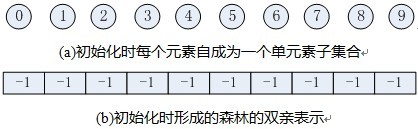
\includegraphics[width=280pt]{ufs1.png}\\
\figcaption{并查集的初始化}\label{fig:ufs1}
\end{center}

\begin{center}
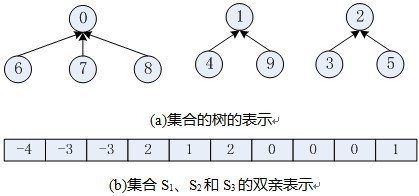
\includegraphics[width=280pt]{ufs2.png}\\
\figcaption{用树表示并查集}\label{fig:ufs2}
\end{center}

\begin{center}
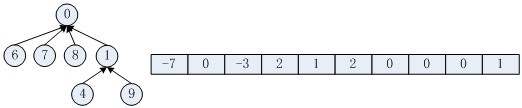
\includegraphics[width=380pt]{ufs3.png}\\
\figcaption{两个集合的并}\label{fig:ufs3}
\end{center}

并查集的C语言实现如下。

\begin{Codex}[label=ufs.c]
/**
 * @brief 初始化并查集.
 * @param[in] s 双亲表示法的数组
 * @param[in] n 数组s的元素个数
 * @return 无
 */
void ufs_init(int s[], int n) {
    int i;
    for(i = 0; i < n; i++) s[i] = -1;
}

/**
 * @brief Find操作.
 * @param[in] s 双亲表示法的数组
 * @param[in] x 要查找的元素
 * @return 包含元素x的树的根
 */
int ufs_find(const int s[], int x) {
    while (s[x] >= 0) {
        x = s[x];
    }
    return x;
}

/**
 * @brief Union操作,求两个不相交集合的并集.
 * @param[in] s 双亲表示法的数组
 * @param[in] root1 一棵树的根
 * @param[in] root2 另一棵树的根
 * @return 如果二者已经在同一集合,并失败,返回0,否则返回1
 */
int ufs_union(int s[], int root1, int root2) {
    if(root1 == root2) return 0;
    s[root1] += s[root2];
    s[root2] = root1;
    return 1;
}
\end{Codex}


\subsection{病毒感染者} %%%%%%%%%%%%%%%%%%%%%%%%%%%%%%
\subsubsection{描述}
一个学校有$n$个社团,一个学生能同时加入不同的社团。由于社团内的同学们交往频繁,如果一个学生感染了病毒,该社团的所有学生都会感染病毒。现在0号学生感染了病毒,问一共有多少个人感染了病毒。

\subsubsection{输入}
输入包含多组测试用例。每个测试用例,第一行包含两个整数$n$,$m$,$n$表示学生个数,$m$表示社团个数。假设$0 < n \leq 30000, 0 \leq m \leq 500$。每个学生从0到$n-1$编号。接下来是$m$行,每行开头是一个整数k,表示该社团的学生个数,接着是$k$个整数表示该社团的学生编号。最后一个测试用例,$n=0,m=0$,表示输入结束。

\subsubsection{输出}
对每个测试用例,输出感染了病毒的学生数目。

\subsubsection{样例输入}
\begin{Code}
100 4
2 1 2
5 10 13 11 12 14
2 0 1
2 99 2
200 2
1 5
5 1 2 3 4 5
1 0
0 0
\end{Code}

\subsubsection{样例输出}
\begin{Code}
4
1
1
\end{Code}

\subsubsection{分析}
非常简单的并查集题目。

\subsubsection{代码}
\begin{Codex}[label=suspects.c]
/* POJ 1611 The Suspects, http://poj.org/problem?id=1611 */
#include <stdio.h>

#define MAXN 30000
int s[MAXN];

/* 等价于复制粘贴,这里为了节约篇幅,使用include,在OJ上提交时请用复制粘贴 */
#include "ufs.c"  /* 见“树->并查集”这节 */

int main() {
    int n, m, k;
    while (scanf("%d%d", &n, &m) && n > 0) {
        ufs_init(s, MAXN);
        while (m--) {
            int x, y; /* 两个学生 */
            int rx, ry; /* x, y 所属的集合的根 */
            scanf("%d", &k);

            k--;
            scanf("%d", &x);
            rx = ufs_find(s, x);
            while (k--) {
                scanf("%d", &y);
                ry = ufs_find(s, y);
                ufs_union(s, rx, ry);  /* 只要是跟x同一个集合的都并进去 */
            }
        }
        /* 最后搜索0属于哪个集合,这个集合有多少人 */
        printf("%d\n", -s[ufs_find(s, 0)]);
    }
    return 0;
}
\end{Codex}

\subsubsection{相关的题目}
与本题相同的题目:
\begindot
\item POJ 1611 The Suspects, \myurl{http://poj.org/problem?id=1611}
\myenddot

与本题相似的题目:
\begindot
\item  None
\myenddot